\documentclass[letterpaper,9pt,twocolumn,twoside,]{pinp}

%% Some pieces required from the pandoc template
\providecommand{\tightlist}{%
  \setlength{\itemsep}{0pt}\setlength{\parskip}{0pt}}

% Use the lineno option to display guide line numbers if required.
% Note that the use of elements such as single-column equations
% may affect the guide line number alignment.

\usepackage[T1]{fontenc}
\usepackage[utf8]{inputenc}

% pinp change: the geometry package layout settings need to be set here, not in pinp.cls
\geometry{layoutsize={0.95588\paperwidth,0.98864\paperheight},%
  layouthoffset=0.02206\paperwidth, layoutvoffset=0.00568\paperheight}

\definecolor{pinpblue}{HTML}{185FAF}  % imagecolorpicker on blue for new R logo
\definecolor{pnasbluetext}{RGB}{101,0,0} %



\title{An Abalone-Age Investigation}

\author[]{470408957 \textbar{} 490443251 \textbar{}}


\setcounter{secnumdepth}{3}

% Please give the surname of the lead author for the running footer
\leadauthor{}

% Keywords are not mandatory, but authors are strongly encouraged to provide them. If provided, please include two to five keywords, separated by the pipe symbol, e.g:
 

\begin{abstract}
In this project we investigated two predictive models for the predicitng
the number of rings in an abalone which is used to find the age by
adding 1.5 to the number. In order for our models to satisfy the
linearity assumptions we had to perform transformations on the data set,
where we then could conduct multiple linear regression through backward
and forward selection using Akaike Information Criterion (AIC). The
resulting model selection was further manipulated as there was strong
observed collinearity with some independant variables which led to our
final model.
\end{abstract}

\dates{This version was compiled on \today} 


% initially we use doi so keep for backwards compatibility
% new name is doi_footer

\pinpfootercontents{pinp Vignette}

\begin{document}

% Optional adjustment to line up main text (after abstract) of first page with line numbers, when using both lineno and twocolumn options.
% You should only change this length when you've finalised the article contents.
\verticaladjustment{-2pt}

\maketitle
\thispagestyle{firststyle}
\ifthenelse{\boolean{shortarticle}}{\ifthenelse{\boolean{singlecolumn}}{\abscontentformatted}{\abscontent}}{}

% If your first paragraph (i.e. with the \dropcap) contains a list environment (quote, quotation, theorem, definition, enumerate, itemize...), the line after the list may have some extra indentation. If this is the case, add \parshape=0 to the end of the list environment.


\section{Introduction}\label{introduction}

The orginal article for this data set was utilised to explore the age of
an abalone. However, the classical method for determining age is to cut
the shell, stain it, and count the number of rings under a microscope.
This is a very tedious process, which provides reasoning to encompass
easier ways in calculating the number of rings without manually counting
the rings. We therefore aim to construct a regression model that can
predict the number of rings an abalone has (calculating the age), using
only an abalones physical attributes which are easily and quickly
measured. To do so, linear relationships need to be considered between
the variables and the value they aim to predict.

\section{Data Set}\label{data-set}

This biological study looks at abalones which are a common type of sea
snail, where the majority of abalone species are found in cold waters,
such as off the coasts of New Zealand, South Africa, Australia, and
Tasmania. The data set is provided by the University of California
Irvine Machine Learning Repository which explores variables describing
physical characteristics for abalones. The original data was collected
by Marine Resources Division in Taroona, Tasmania, containing 4177
observations with 9 different variables which has no missing values.

\subsection{2.1 Variables}\label{variables}

\begin{itemize}
     \item[$-$] Sex; factor; male, female or infant
     \item[$-$] Length (mm); continous; longest shell measurement
     \item[$-$] Diameter (mm); continous; perpendicular to length
     \item[$-$] Height (mm); continous; with meat in shell
     \item[$-$] Whole Weight (g); continous; whole abalone
     \item[$-$] Shucked Weight (g); continous; weight of meat
     \item[$-$] Viscera Weight (g); continous; gut weight (after bleeding)
     \item[$-$] Shell Weight (g); continous; after being dried
     \item[$-$] Rings; integer; number of rings. +1.5 gives age in years
\end{itemize}

\subsection{2.2 Outliers}\label{outliers}

In exploring the different variables there appeared to be two values
identified as clear outliers in the height variable. Thus, concluding
they are likely to be errors induced when entering the data and will be
filtered out.

\begin{center}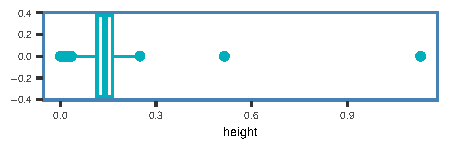
\includegraphics{ExecSum_files/figure-latex/unnamed-chunk-1-1} \end{center}

\section{Analysis}\label{analysis}

\subsection{3.1 Transformations}\label{transformations}

Prior to selecting an appropriate model, with reference to appendix 1,
clearly the indepedant variables do not possess a linear relationship
with number of rings. The variables clearly rise rapidly and reach a
plateau, thus it was found best to perform log transformations of the
variable rings, length, diameter, weight shucked, weight viscera, weight
shell and a square root transformation was applied to height and log of
rings. With reference to appendix 2, the data set now adopts a linear
relationship with the predictive variable, allowing for a linear
regressive model to work appropiately.

\subsection{3.2 Model Selection}\label{model-selection}

Provided the linearity assumptions with respect to the dependant
variable are satisfied, a model search was justfiied by the Akaike
information criterion through a backward and forward variable seleciton.
After conducting the relevant seacrch it was found that the forward
model did not include log of diameter and log of length while the
backward approach included all variables, shown in the table below.

\begin{center}
\begin{tabular}{c c c c c}
    & Forward Model & & Backward Model & \\
    \hline
    Predictors & Estimates & p & Estimates & p\\
    \hline
    (Intercept) & 1.43 & $\textbf{<0.001}$ & 1.45 & $\textbf{<0.001}$\\
    log shell & 0.11 & $\textbf{<0.001}$ & 0.11 & $\textbf{<0.001}$\\
    logshucked & -0.19 & $\textbf{<0.001}$ & -0.19 & $\textbf{<0.001}$\\
    logwhole & 0.19 & $\textbf{<0.001}$ & 0.20 & $\textbf{<0.001}$\\
    sexi & -0.02 & $\textbf{<0.001}$ & -0.01 & $\textbf{<0.001}$\\
    logviscera & -0.03 & $\textbf{<0.001}$ & -0.02 & $\textbf{<0.001}$\\
    sqrtheight & 0.13 & $\textbf{0.007}$ & 0.12 & $\textbf{0.012}$\\
    logdiam &  & & 0.07 & $\textbf{0.005}$\\
     loglength &  & & -0.08 & $\textbf{0.005}$\\
    \hline
    Observations & 4175 &  & 1.45 & \\
    $R^2/R^2$ adjusted & 0.647 / 0.647 & & 0.648 / 0.647 & \\
    AIC & -10882.310 & & -10887.886 & \\
\end{tabular}
\end{center}

 \#\# 3.3 Assumption Checking

\subsubsection{Forward Residual Verse Fitted/QQ
Plot}\label{forward-residual-verse-fittedqq-plot}

\begin{center}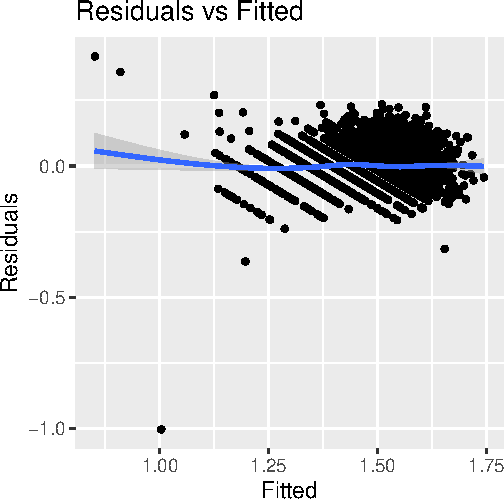
\includegraphics{ExecSum_files/figure-latex/unnamed-chunk-4-1} \end{center}

\subsubsection{Backward Residual Verse Fitted/QQ
Plot}\label{backward-residual-verse-fittedqq-plot}

\begin{center}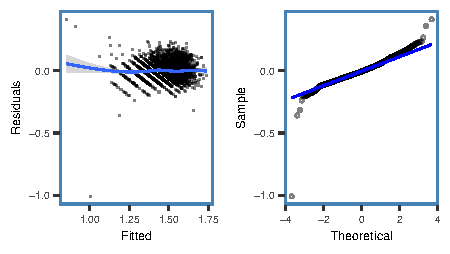
\includegraphics{ExecSum_files/figure-latex/unnamed-chunk-5-1} \end{center}

Assumption checks for both forward and backward models;

\begin{figure}[!h]
    \begin{center}
    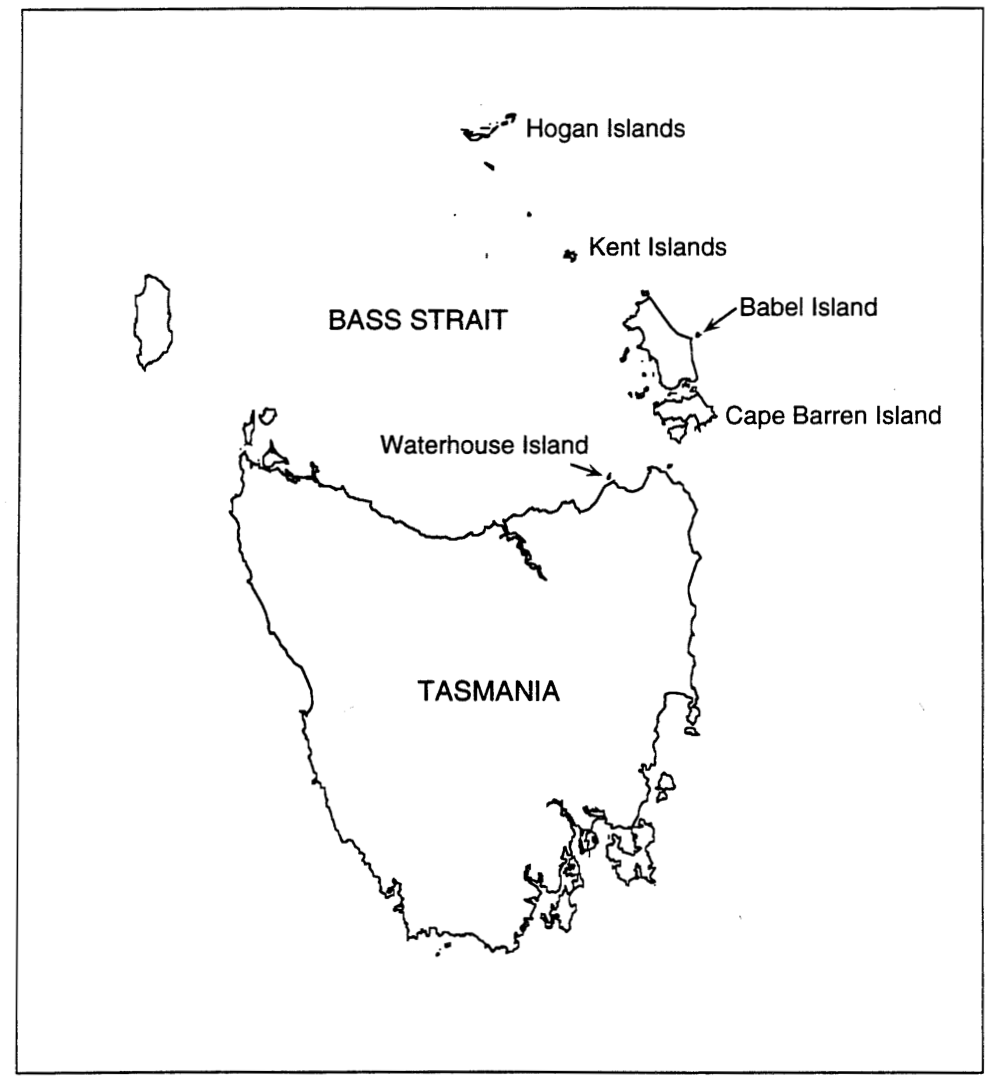
\includegraphics[width=0.3\textwidth, height=1.8in]{Independence} 
    \end{center}
\end{figure}

\begin{itemize}
     \item[$-$] \textbf{Linearity}: The residual vs fitted values plot indicates no obvious curvature for both thus the linearity assumption is satisfied.
     \item[$-$] \textbf{Independence}: Referencing to appendix 3 the data was collected over 5 different regions in the Tasman Sea, hence there will be independence between the observations from the differing locations that the data was pulled from.
     \item[$-$] \textbf{Homoskedasticity}: The residuals do not appear to be fanning out or changing over the range of the fitted values for both, thus the constant error variance assumption is met.
     \item[$-$] \textbf{Normality}: The normality assumption is at least approximately satisfied. In the QQ plot, the points are reasonably close to the diagonal line, however the sample size is large enough to rely upon the central limit theorem ensuring the inferences are approximately valid.
\end{itemize}

\section{Results}\label{results}

They had the same adjusted R\^{}2 thus we need to encompass the RMSE and
MAE to identify the better performing model. Cross validation was used
to compute RMSE and MAE of our forward and backward models. This is done
to account for and minimise overfitting. From comparing the two models'
RMSE and MAE we could see that they only differ very slightly,
indicating the better performing model will be the backward model over
the forward model, due to having a lower RMSE and MAE.

\begin{center}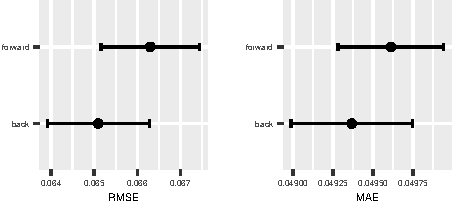
\includegraphics{ExecSum_files/figure-latex/unnamed-chunk-8-1} \end{center}

Talk about Given the strong multicollinearity observed between some
variables it is good to note the multicollinearity among some variables,
does it make sense to include all the weight variables in the model?
There is no mention of the observed collinearity and its effect on the
model.

\section{Discussion/Conclusion}\label{discussionconclusion}

All standard LaTeX environment are directly usable if needed, including
of course all mathematical environments and symbols such as, say, the
greek lettering: \(\alpha\), \(\beta\), \(\gamma\), and so on.

%\showmatmethods

\pnasbreak 



\begin{thebibliography}{3}
\newcommand{\enquote}[1]{``#1''}
\providecommand{\natexlab}[1]{#1}
\providecommand{\url}[1]{\texttt{#1}}
\providecommand{\urlprefix}{URL }
\expandafter\ifx\csname urlstyle\endcsname\relax
  \providecommand{\doi}[1]{doi:\discretionary{}{}{}#1}\else
  \providecommand{\doi}{doi:\discretionary{}{}{}\begingroup
  \urlstyle{rm}\Url}\fi
\providecommand{\eprint}[2][]{\url{#2}}

\bibitem[{Allaire \emph{et~al.}(2017)Allaire, {R Foundation}, Wickham, {Journal
  of Statistical Software}, Xie, Vaidyanathan, {Association for Computing
  Machinery}, Boettiger, {Elsevier}, Broman, Mueller, Quast, Pruim, Marwick,
  Wickham, Keyes, and Yu}]{CRAN:rticles}
Allaire J, {R Foundation}, Wickham H, {Journal of Statistical Software}, Xie Y,
  Vaidyanathan R, {Association for Computing Machinery}, Boettiger C,
  {Elsevier}, Broman K, Mueller K, Quast B, Pruim R, Marwick B, Wickham C,
  Keyes O, Yu M (2017).
\newblock \emph{rticles: Article Formats for R Markdown}.
\newblock R package version 0.4.1,
  \urlprefix\url{https://CRAN.R-project.org/package=rticles}.

\bibitem[{MacFarlane(2017)}]{pandoc}
MacFarlane J (2017).
\newblock \emph{Pandoc: A Universal Document Converter}.
\newblock Version 1.19.2.1, \urlprefix\url{http://pandoc.org}.

\bibitem[{Xie(2017)}]{CRAN:knitr}
Xie Y (2017).
\newblock \emph{knitr: A General-Purpose Package for Dynamic Report Generation
  in R}.
\newblock R package version 1.17, \urlprefix\url{https://yihui.name/knitr/}.

\end{thebibliography}

\end{document}

